\usetikzlibrary{angles}

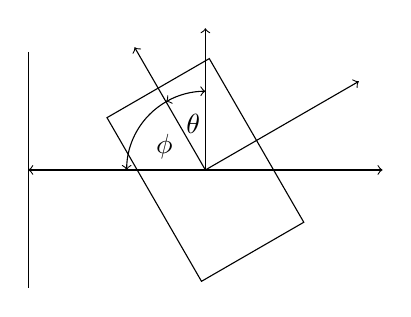
\begin{tikzpicture}[scale=3]
	\draw (0,1) -- (0,0);

	\begin{scope}[shift={(.5,.1)},rotate around={30:(.25,.4)}]
		\draw (0,0) rectangle (.5,.8);
		\draw[<->] (.25,1) coordinate (A) -- (.25,.4) -- (1,.4);

		\draw[<->,rotate around={-30:(.25,.4)}] (.25,1) coordinate (C) 
			-- (.25,.4) coordinate (B) -- (1,.4) 
			pic[pic text=$\theta$,draw,angle radius=1cm] {angle=C--B--A};
	\end{scope}

	\draw[->] (.75,.5) -- (0,.5) coordinate (D)
		pic[pic text=$\phi$,draw,angle radius=1cm] {angle=A--B--D};

\end{tikzpicture}
